\documentclass[12pt,letterpaper]{article}

\newcommand\hwnumber{C3M3}
\usepackage{fullpage}
\usepackage[top=2cm, bottom=4.5cm, left=2.5cm, right=2.5cm]{geometry}
\usepackage{amsmath,amsthm,amsfonts,amssymb,amscd}
\usepackage{lastpage}
\usepackage{enumerate}
\usepackage{fancyhdr}
\usepackage{mathrsfs}
\usepackage{xcolor}
\usepackage{graphicx}
\usepackage{listings}
\usepackage{hyperref}
\usepackage{enumitem}


\hypersetup{%
  colorlinks=true,
  linkcolor=blue,
  linkbordercolor={0 0 1}
}
% Reduce whitespace around figures
\setlength\intextsep{0pt}
 
 \newcommand{\twolines}{\vspace{5em}}
 \newcommand{\smallspace}{\vspace{12em}}
 \newcommand{\bigspace}{\vspace{60em}}
 
\renewcommand\lstlistingname{Algorithm}
\renewcommand\lstlistlistingname{Algorithms}
\def\lstlistingautorefname{Alg.}

\lstdefinestyle{Python}{
    language        = Python,
    frame           = lines, 
    basicstyle      = \footnotesize,
    keywordstyle    = \color{blue},
    stringstyle     = \color{green},
    commentstyle    = \color{red}\ttfamily
}

\setlength{\parindent}{0.0in}
\setlength{\parskip}{0.05in}
\setlist{leftmargin=2.5mm}

% Edit these as appropriate
\newcommand\course{CMPUT 397}


\pagestyle{fancyplain}
\headheight 35pt

\chead{\textbf{\Large Worksheet \hwnumber}}
\rhead{\course \\ \today}
\lfoot{}
\cfoot{}
\rfoot{\small\thepage}
\headsep 1.5em


\begin{document}

\begin{enumerate}
	\item (\textit{Exercise 10.2 S\&B})
Give pseudocode for semi-gradient one-step Expected Sarsa for control. You can build on the semi-gradient Sarsa code for this question.
%
\begin{figure}[h!]
  \center
  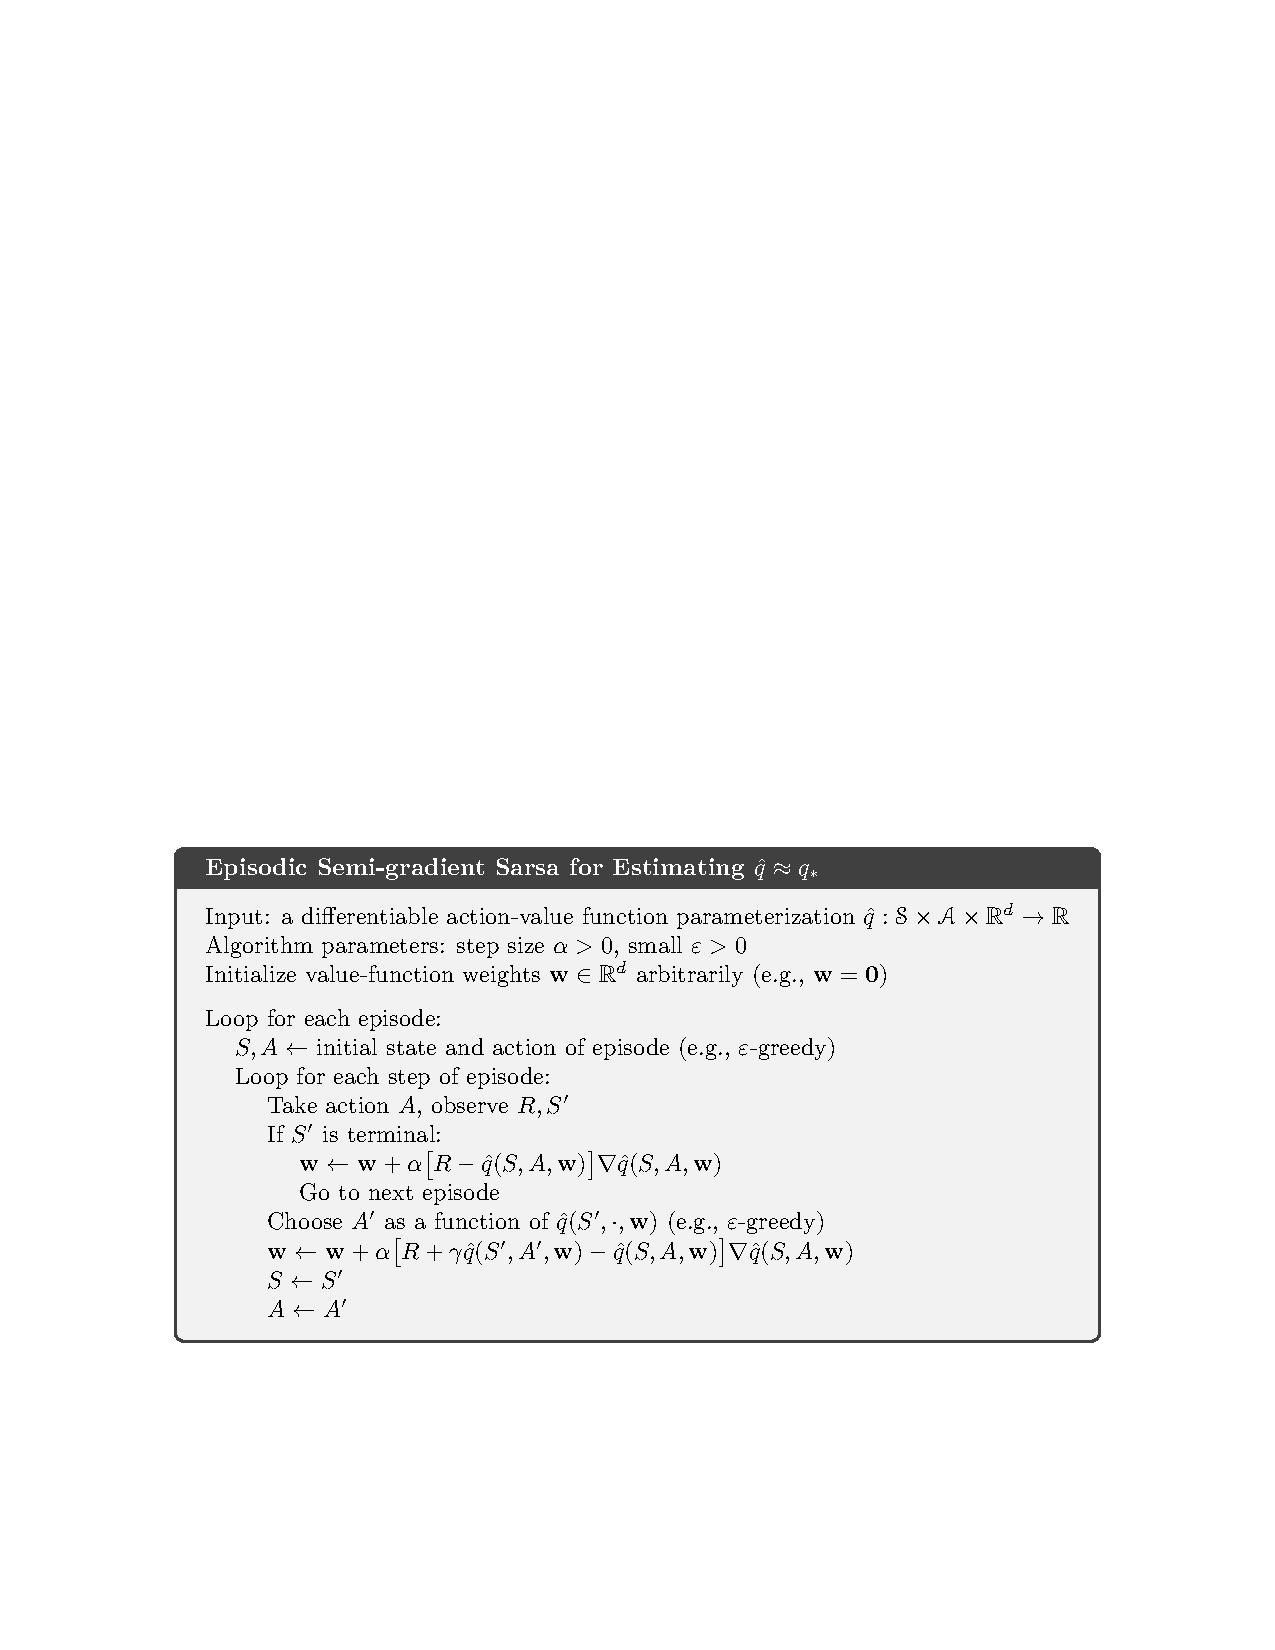
\includegraphics[width=0.75\linewidth]{figures/semisarsa.pdf}
\end{figure}
%
	\item (\textit{Exercise 10.1 S\&B})
We have not explicitly considered or given pseudocode for any Monte Carlo
methods in this chapter. What would they be like? Why is it reasonable not to give
pseudocode for them? 
%How would they perform on the Mountain Car task?
		\item How would you use optimistic initial values, for Sarsa with a tile coding function approximator? Assume you have a two dimensional input, and you use $m$ tilings, and $n$ tiles, to give $m$ grids of size $n \times n$ resulting in $m \times n \times n$ features. What size is your weight vector? And how do you initialize your weights to ensure you have optimistic initial values? Assume the maximum reward is $R_\text{max}$ and we use a $\gamma < 1$.

	% MARTHAC: This uses n-step returns, which we don't cover
%	\item (\textit{Exercise 10.3 S\&B})
Why do the results shown in Figure 10.4 have higher standard errors at
large $n$ than at small $n$?
% MARTHAC: Let's not emphasize differential algs, since we wont use them
%	\item (\textit{Exercise 10.4 S\&B})
Give pseudocode for a differential version of semi-gradient Q-learning.
%	\item (\textit{Exercise 10.5 S\&B})
What equations are needed, in addition to the equation below,
$$\delta_{t} = R_{t+1} - \bar R_{t} + \hat v (S_{t+1}, \mathbf{w}_{t}) - \hat v (S_{t}, \mathbf{w}_{t})$$
to specify the differential version of $TD(0)$?
% MARTHAC: Way too advanced
%	\item Suppose there is an MDP that under any policy produces the deterministic
sequence of rewards $+1, 0, +1, 0, +1, 0, \dotso$ going on forever. Technically, this is not allowed
because it violates ergodicity; there is no stationary limiting distribution $\mu_{\pi}$ and the limit
$$\underset{t\rightarrow \infty}{\lim} \mathbb{E}[R_{t} | S_{0}, A_{0:(t-1)} \sim \pi]$$
does not exist. Nevertheless, the average reward,
$$\underset{h\rightarrow \infty} {\lim}\frac{1}{h} \sum_{t=1}^{h}\mathbb{E}[R_{t} | S_{0}, A_{0:(t-1)} \sim \pi]$$
is well defined;
What is it? Now consider two states in this MDP. From A, the reward sequence is exactly as described above, starting with a $+1$, whereas, from B, the reward sequence starts with a $0$ and then continues with $+1, 0, +1, 0,\dotso $ The differential return
$$G_{t} = R_{t+1} - r(\pi) + R_{t+2} - r(\pi) + R_{t+3} - r(\pi) + \, \dotso$$
is not well defined for this case as the limit does not exist. To repair this, one could alternately define the value of a state as

$$ v_{\pi} = \underset{\gamma \rightarrow 1}{\lim}\, \underset{h \rightarrow \infty}{\lim} \sum_{t=0}^{h} \gamma^{t}\left(  \mathbb{E}_{\pi} [R_{t+1} | S_{0} = s] - r(\pi)\right)$$
Under this definition, what are the values of states A and B?
% MARTHAC: We just have too many question, but this one *could* be added back
%	\item (\textit{Exercise 10.7 S\&B})
Consider a Markov reward process consisting of a ring of three states A, B,
and C, with state transitions going deterministically around the ring.
A reward of $+1$ is received upon arrival in A and otherwise the reward is $0$.
What are the differential values of the three states using
$$ v_{\pi} = \underset{\gamma \rightarrow 1}{\lim}\,\, \underset{h \rightarrow \infty}{\lim} \sum_{t=0}^{h} \gamma^{t}\left(  \mathbb{E}_{\pi} [R_{t+1} | S_{0} = s] - r(\pi)\right)$$
	\item (\textit{Exercise 10.8 S\&B})
The pseudocode in the box on page 251 updates $\bar R_{t}$ using $\delta_{t}$ as an error rather than simply $R_{t+1} -  \bar R_t$.
Both errors work, but using $\delta_{t}$ is better.
To see why, consider the ring MRP of three states from Exercise 10.7.
\begin{figure}
  \center
  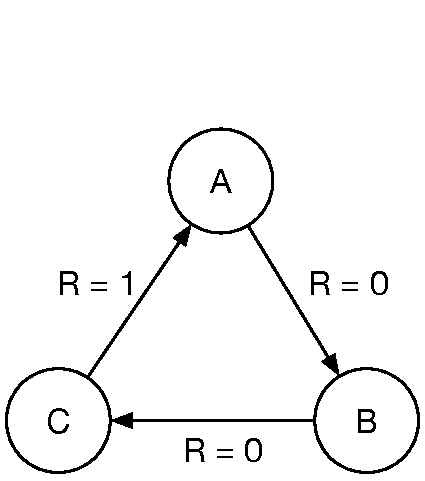
\includegraphics[width=0.2\linewidth]{figures/10dot8.pdf}
\end{figure}
The estimate of the average reward should tend towards its true value of $\frac{1}{3}$.
Suppose you fix $\bar R_{t} = \frac{1}{3}$ and fix $v_{\pi}(A) = \frac{-1}{3}, v_{\pi}(B) = 0, v_{\pi}(C) = \frac{1}{3}$, which are the true values.
What is the sequence of $R_{t+1} - \bar R_{t}$ errors, when going from A to B, B to C and then C to A?
Correspondingly, what is the sequence of TD errors? Here, since we use the true values, we have
$\delta_{t} = R_{t+1} - \bar R_{t} + v_{\pi} (S_{t+1}) - v_\pi (S_{t})$. 
What does this tell us about which error sequence would produce a more stable estimate of the average reward if the estimates were allowed to change in response to the errors? Why?

\end{enumerate}

\end{document}
%%% Local Variables:
%%% mode: latex
%%% TeX-master: t
%%% End:
